\begin{center}
	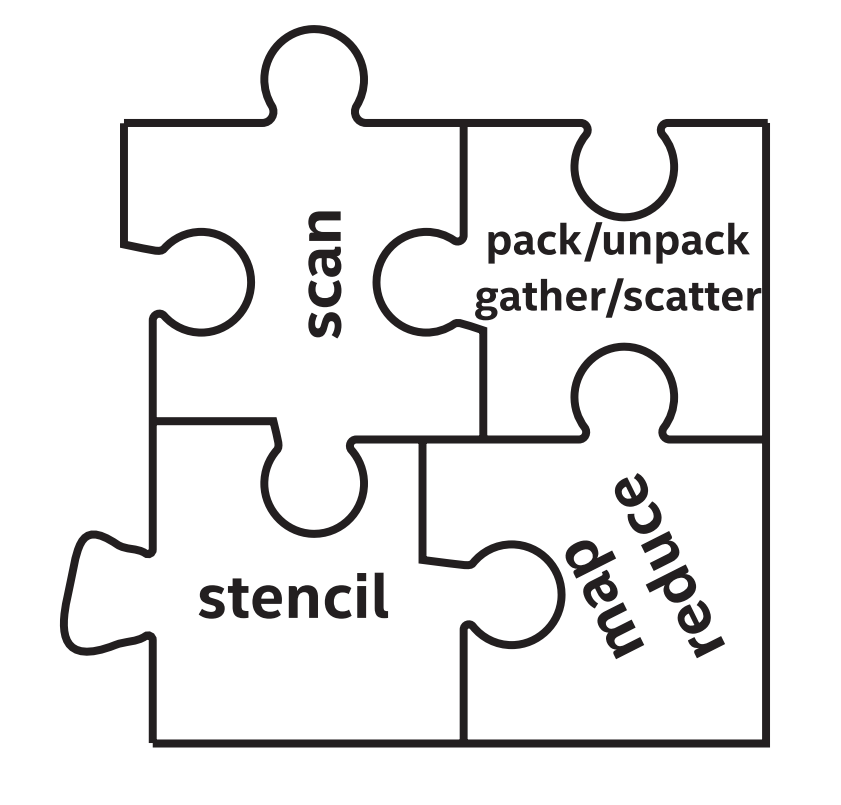
\includegraphics[width=0.5\textwidth]{content/chapter-14/images/1}
\end{center}

当我们处于最佳状态时,在工作中认识到模式,并证明其是最佳解决方案的技术。并行编程也不例外,需要研究和研究已有的模式。考虑大数据应用中采用的MapReduce框架,他们的成功很大程度上是基于两个简单而有效的并行模式——map和reduce。\par

并行编程中有很多常见的模式,与我们的编程语言无关。这些模式是通用的,可以进行任何级别的并行(例如:子工作组、工作组、设备)和任何设备(例如:CPU, GPU, FPGA)上使用。但是,模式的某些属性(例如可扩展性)可能会影响其对不同设备的适用性。某些情况下,使应用程序适应新设备可能只需要选择适当的参数或微调模式的实现,我们可以通过选择完全不同的模式来提高性能。\par

理解如何、何时以及在何处使用这些常见的并行模式是提高对DPC++(以及一般的并行编程)熟练程度的关键部分。对于那些具有并行编程经验的人来说,了解这些模式是如何在DPC++中表达的,可以快速了解并熟悉该语言的功能。\par

本章旨在解答以下问题:\par

\begin{itemize}
	\item 理解哪些模式是最重要的?
	\item 模式如何与不同设备的功能相关联?
	\item 哪些模式已经作为DPC++函数和库提供?
	\item 如何使用直接实现模式?
\end{itemize}










